\section{Gas Detector construction}

\subsection{Cider can}
\subsubsection{Material preparation}
We have been handed a start-up kit consisting of one empty \SI{500}{\milli\liter}
cider can, two plexiglas endcaps, two teflon pipes, one nylon screw and nut,
brass pipes and a high voltage (HV) connector with a small exterior connector for
grounding the outside of the can.

The process started with the preparation of the cider can which included cutting
away the top part of the can, removing the inner coating with a drill equipped with a
metal brush on top, drilling a two holes in the bottom, on the the middle of the
bottom part for the nylon screw and one in one side of the bottom part for the
gas exchange system (of $d = \SI{8.0}{\milli\meter}$ and $d =
\SI{6.0}{\milli\meter}$). The second step consisted in drilling the necessary
holes in the plexiglas endcaps (which already have a groove for the can
extremities to be fitted in), one hole for the gas teflon pipe in the back
endcap and one in the front endcap as well as a hole for the HV connector in the
front endcap (the diameters are $d = \SI{6.0}{\milli\meter}$ and $d =
\SI{9.5}{\milli\meter}$ respectively). Finally a small hole of $d =
\SI{1.0}{\milli\meter}$ was drilled in the teflon screw, in order to fit the
brass pipe in there at a later point. The brass tubes were cut and flattened
with sand paper, to remove the part that was squeezed due to the cutting tool.

\begin{figure}[h]
  \centering
  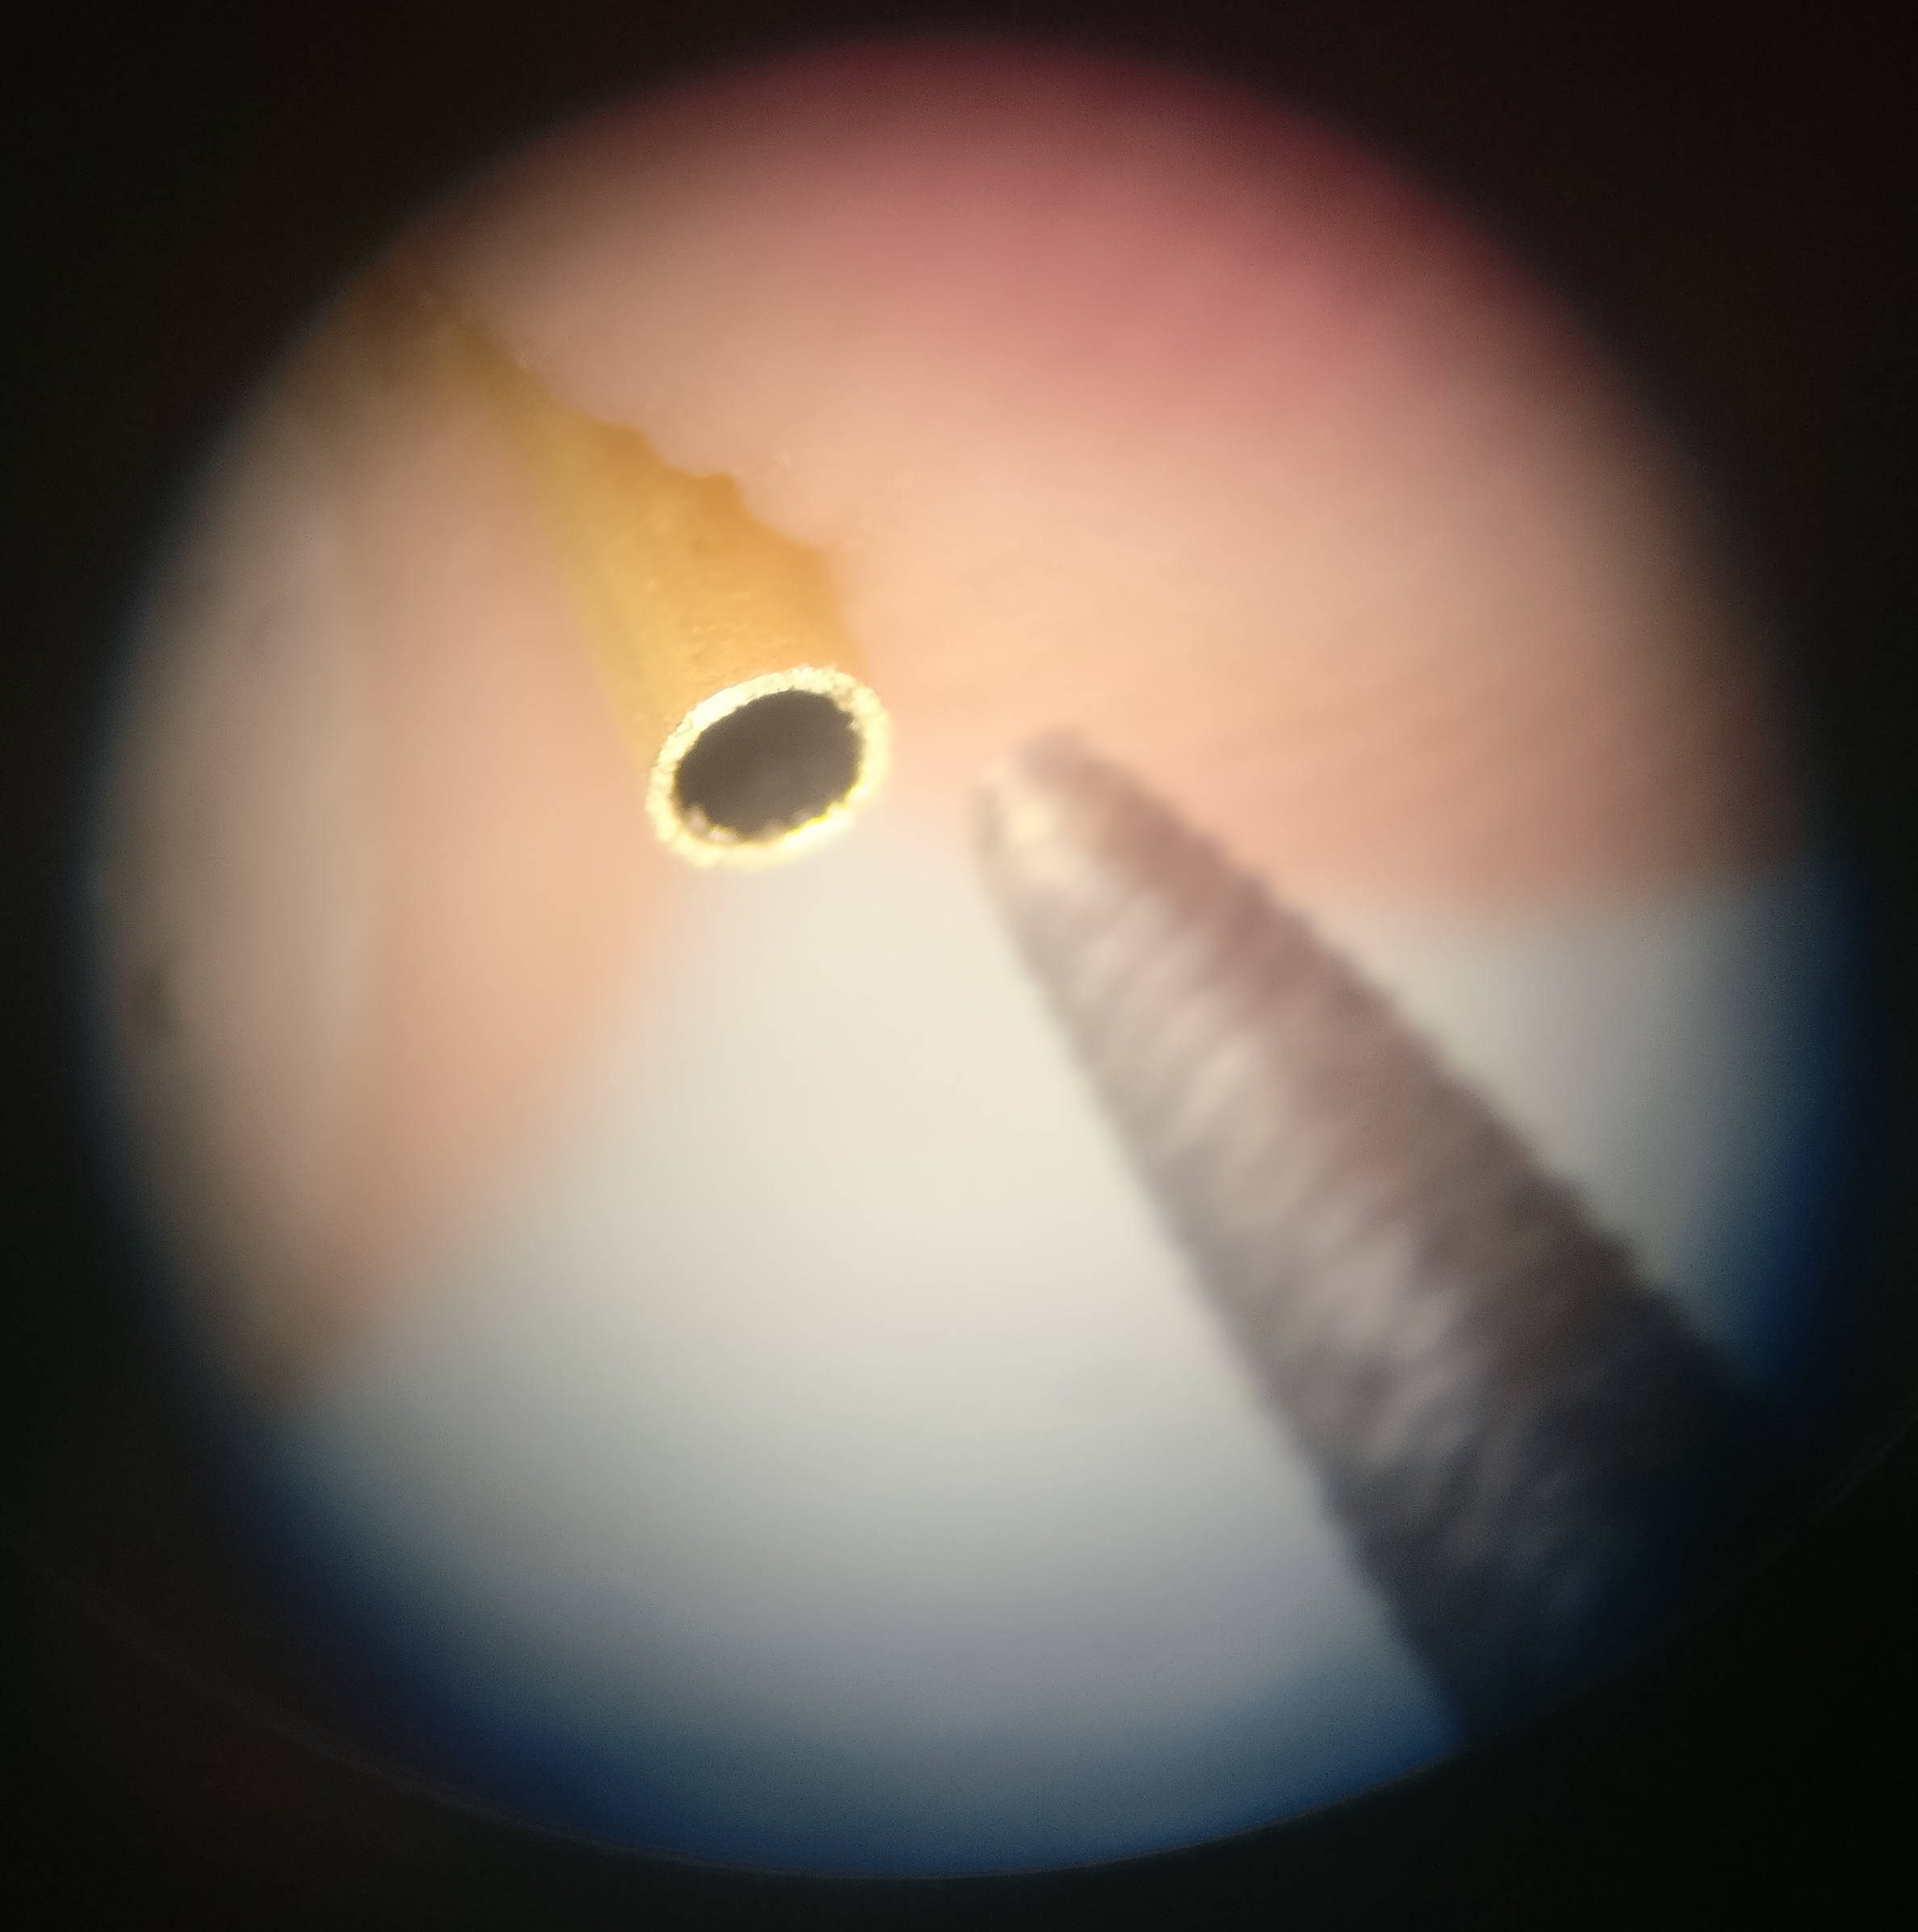
\includegraphics[width=0.8\textwidth]{./graphics/brass_file.jpg}
  \caption{Filing of the brass tube}
  \label{fig:brass_file}
\end{figure}


Once all the ingredients were ready, all the holes in the can and the edges of
the brass tube were filed and checked under a microscope (see \ref{fig:brass_file}), in order to avoid
sharp edges. All the components were placed in an isopropanol (IPA) bath in a
sonicator, so all the skin oils and dirt were cleaned off, and the parts were
dried with $\mathrm{N}_2$ gas. At this point the only element missing was the
anode wire, which was taken from a regular low voltage cable and carefully wiped
with a cloth dipped in IPA.


\subsubsection{Assembly}

The assembly of the detector commenced with the fastening of the nylon screw and
bolt to the aluminium can through the hole in the middle of the bottom of the
can. The longer of the two brass tubes was inserted in the nylon screw and one
end of the anode wire was passed in the brass tube from the outside and pulled
until the other end of the can. On the other extremity of the anode wire, a
small nut was attached with a simple nod, in order to help keeping the anode
wire straight later on in the process. The free end of the wire was inserted in
the shorter brass tube and they were both soldered to the HV connector, which
had been previously fastened to the front plexiglass endcap (and a small contact
has been placed between the HV connector and the outer glass, in order to later
use it for grounding the cathode). The front endcap was glued with epoxy to the
cider can and was left to dry for some time. The next step consisted in
straightening out the anode wire inside the can by pulling it slowly out of the
can from the bottom. The wire has to be quite straight in order to avoid dips,
where the charge could concentrate and ocscure the measurement. To reach an
optimal condition, a weight was applied to the wire as well as careful tension.
When a satisfactory straightness was achieved, the wire was soldered to the
brass pipe and the rest cut off. The back endcap was glued to the cider can and
left to dry for some time.

The gas teflon tubes were glued to the front and back endcap and a small
quantity of glue was applied around the HV connector, to insure optimal
insulation.

Before moving on to the next step, a leakage test was performed, to check for
possible holes in the glue. The gas supply (in our case $\mathrm{P}_{10}$) was
attached to one of the teflon gas tubes and to a flowmeter, which measured a gas
flow of approximately \SI{25}{\milli\liter\per\minute} out of the tube. When
moving the flowmeter to the other end of the can detector, the gas flow measured
was between \SIrange{2}{4}{\milli\liter\per\min}, which meant that an extra layer
of glue had to be applied to the outside and the endcaps and to the tube
connections, to cover for the leakage/leakages. After this adjustment, the gas
flow was measured again and the gas flow injected in the detector was
\SI{18.3}{\milli\liter\per\minute}, while the outgoing gas flow was of
\SI{17.6}{\milli\liter\per\minute}, which was determined sufficient for the
purpose of the experiment.

The last step consisted in removing some of the coating from the outside of the
cider can with sand paper and connecting the grounding pin previously attached
to the HV connector to the bare aluminuium of the can with a copper tape, to
later ground the cathode to create the electric field inside the can. The
connection was checked with a multimiter, where it was asserted, that there is
no connection between the cathode can and the anode wire.

\subsection{Copper Tube}
\subsubsection{Assembly}
Following the more rudimentary cider can detector, a more sophisticated detector made out of copper was built. In this iteration of the gas counter, the  proportional chamber experiment was made out of a machined copper tube. The end caps were made out of two teflon plugs, brass tubes were again used as electric field protector, and a finer, copper beryllium wire was selected as the anode material. The material also included smalelr teflon pipes for the gas inlets, and the same HV connector and a the same grounding pin as the cider can assembly. Figure \ref{fig:copper_parts} shows all parts of the assembly.

Similarly to the previous detector, the brass pipe was sanded and filed at the edges to remove any sharp debris that would cause sparking.

In order to ensure that the X-ray emission from the source would be able to penetrate the thicker walls of the copper tube, a hole of $5$ mm was drilled in the copper tube, approximately in the middle of the pipe. The teflon plugs were filed down in order to match the inner radius of the copper pipe and the pre-existent holes for the gas supply tubes. The HV connector and brass tube were adjusted to the appropriate sizes of the different components. Similarly to the previous detector, the brass pipe was sanded and filed at the edges to remove any sharp debris that would cause sparking.

All the parts were cleaned in a IPA bath and dried with N$_2$. The wire was soldered to the brass tube and to the HV connector and inserted carefully in the copper tube. This part of the procedure was much more delicate than in the previous assembly, given the tendency of the much thinner wire to curl on itself and break easily. The copper tube was glued with epoxy to the front teflon plug. The wire was then passed into the second brass tube and in the back teflon plug  The back plug was glued and the wire soldered to the brass tube.

\begin{figure}[h]
  \centering
  \includegraphics[width=0.8\textwidth]{./graphics/copper_tube_parts.jpg}
  \caption{Cleaned parts of the copper tube assembly}
  \label{fig:copper_parts}
\end{figure}

Finally, the hole drilled for the target was covered by a small piece of metallic tape, held in place by epoxy glue to seal off the opening.

\subsubsection{Testing}

The copper tube detector was flushed and then filled with P10 gas and connected to the amplifier electronics in a similar fashion than the previous detector. Unfortunately, preliminary observations of the signal at the oscilloscope indicated a problem with the state of the detector, as no pulses appeared on the screen event in the presence of a radioactive source. Further investigation led us to realie that the HV connector became shorted when leftover parts of the anode wire (that did not get cut) came into contact with the outer part of the connector as the end cap was inserted into the tube. This rendered the device inoperable, and thus we neede to rely on measurements on reference tubes to get a comparison with the can detector. Results in section \ref{sec:special_detec} have thus not been made with the instrument characterized in table \ref{table:copper}.
